\paragraph*{2.2 Прямая задача кинематики}$\phantom{-}$\\
\hspace*{\parindent} Прямая задача кинематики (ПЗК) заключается в вычислении координат системы, связанной со схватом (рабочим инструментом), в зависимости от обобщенных координат манипулятора.\\
\hspace*{\parindent}Для решения ПЗК рассматриваются две системы координат: исходная, связанная с «землей» $o_0 x_0 y_0 z_0$ и итоговая, связанная с рабочим инструментом $o_n x_n y_n z_n$. Как известно, расположение этих двух систем друг относительно друга определяется тремя линейными и тремя угловыми координатами.\\
\hspace*{\parindent}Итак, рассмотрим подробнее переход между обобщенными и глобальными координатами. Данный переход можно представить в виде: $k^0 = T_n^0 k^n$, 

где $T_n^0$ - матрица преобразования, несущая информацию о линейном смещении и пространственной ориентации одной системы относительно другой.\\


\begin{equation*}\label{eq:model}
T_n^0=
    \begin{bmatrix}
    n_x & s_x & a_x & p_x \\
    n_y & s_y & a_y & p_y \\
    n_z & s_z & a_z & p_z \\
    0 & 0 & 0 & 1 \\
    \end{bmatrix}
    =
     \begin{bmatrix}
    n_n^0  &  s_n^0 & a_n^0 & p_n^0 \\
    0 & 0 & 0 & 1\\
    \end{bmatrix}
     =
     \begin{bmatrix}
    R_n^0  &  p_n^0 \\
     0 & 1\\
    \end{bmatrix}
    ,\\
\end{equation*} 

\hspace*{\parindent} где векторы  $n_n^0$,  $s_n^0$ и $a_n^0$ выражают направления осей $x_n$, $y_n$ и $z_n$, О O соответственно, относительно системы координат $o_0 x_0 y_0 z_0$, $R_n^0 \in$ SO - матрица 3х3 вращения системы  $o_n x_n y_n z_n$ относительно $o_0 x_0 y_0 z_0$, $p_n^0$ $\in$ $R^3$ - вектор линейного смещения начала координат системы  $o_n x_n y_n z_n$ относительно $o_0 x_0 y_0 z_0$.\\
\hspace*{\parindent} матрица $T_n^0$ имеет размерность 4х4, значит нужно расширить векторы координат $v^0$ и $v^n$ единицей для соответствия размерностей в матричных уравнениях:\\
\begin{equation*}\label{eq:model}
     \begin{bmatrix}
     x^0 \\
     y^0\\
     z^0\\
     1\\
    \end{bmatrix}
     =T_n^0
     \begin{bmatrix}
     x^n \\
     y^n\\
     z^n\\
     1\\
    \end{bmatrix}
    .\\
\end{equation*} 
\newpage 
\hspace*{\parindent} Рассмотрим самые важные свойства, характеристики и отдельные элементарные компоненты, которые будут активно использоваться в пособии:\\

1. Поворот на нулевой угол определяется единичной матрицей\\
\begin{equation*}\label{eq:model}
R_{\beta=0} = 
     \begin{bmatrix}
    1 & 0 & 0\\
    0 & 1 & 0\\
    0 & 0 & 1\\
    \end{bmatrix}
     =I
\end{equation*} 

2. Поворот в отрицательном направлении определяется
\begin{equation*}\label{eq:model}
R_{-\beta} = R_{\beta}^{-1} = R_{-\beta}^T
\end{equation*} 

3. Существуют так называемые базовые матрицы вращения вокруг осей x, y и z:
\begin{equation*}\label{eq:model}
R_{x, \beta} = 
     \begin{bmatrix}
    1 & 0 & 0\\
    0 & cos\beta & -sin\beta\\
    0 & sin\beta & cos\beta\\
    \end{bmatrix}
    , \\
\end{equation*} 

\begin{equation*}\label{eq:model}
R_{y, \beta} = 
     \begin{bmatrix}
    cos\beta & 0 & sin\beta\\
    0 & 1 & 0\\
    -sin\beta & 0 & cos\beta\\
    \end{bmatrix}
    , \\
\end{equation*} 

\begin{equation*}\label{eq:model}
R_{z, \beta} = 
     \begin{bmatrix}
   
    cos\beta & -sin\beta & 0\\
    sin\beta & cos\beta & 0\\
    0 & 0 & 1\\
    \end{bmatrix}
    , \\
\end{equation*} 
где $\beta$ - некоторый угол.\\

\hspace*{\parindent} Рассмотрим вывод матрицы $R_{z,\theta}$\\
\hspace*{\parindent}В трехмерной системе координат каждая ось системы $x
_1y_1z_1$ проецируется на систему координат $x_0y_0z_0$. Результирующая матрица вращения задается как

\begin{equation*}\label{eq:model}
R_1^0 = 
     \begin{bmatrix}
x_1x_0 & y_1x_0 & z_1x_0 \\
x_1y_0 & y_1y_0 & z_1y_0\\
x_1z_0 & y_1z_0 & z_1z_0\\
    \end{bmatrix}
    , \\
\end{equation*} 

\hspace*{\parindent}Полученная матрица 3 × 3 в этой форме ортогональна, ее определитель равен единице. 
\begin{center}
    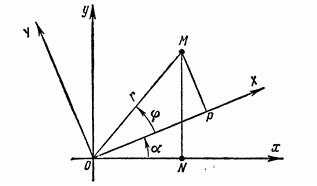
\includegraphics[width=0.8\textwidth]{Lab3/pictures/rotation.png}\\
    Рисунок 2.2.1 Старая система и новая системы координат\\
\end{center}
\hspace*{\parindent} Рассмотрим две системы координат, заданные на плоскости, с общим началом в точке О: исходная система Oxy и новая OXY, которая повёрнута на угол между осями Ox и OX, равный $\alpha$ (угол между осями Oy и OY также равен $\alpha$). Выведем формулы, которые выражают старые координаты x и y точки М, выбранной произвольным образом, через ее новые координаты X и Y.\\
Для этого перейдем в полярные координаты: у старой системы координат полярная ось совпадает с Ox, а у новой - с OX. Пусть у точки М в новой полярной системе координат будет полярный угол $\phi$ и полярный радиус r. Тогда, в старой полярной системе полярный угол точки М= $\phi+\alpha$, а радиус останется тем же.\\
Таким образом: \\
$x=rcos(\alpha+\phi)$,\\
$y=rsin(\alpha+\phi)$.\\
С использованием тригонометрических тождеств и суммы двух углов, получаем:\\
$x=r(cos\alpha cos\phi - sin \alpha sin \phi) = (rcos \phi)cos \alpha - (rsin\phi)sin\alpha$\\
$y=r(sin\alpha cos\phi + cos \alpha sin\phi) = (rcos\phi)sin\alpha + (rsin\phi)cos\alpha$\\
Т.к. $rcos\phi$ = X и $rsin\phi$ = Y, получаем:\\
\begin{equation*}
 \begin{cases}
x=Xcos\alpha - Ysin\alpha,\\
y=Xsin\alpha + Ycos\alpha.\\
 \end{cases}
\end{equation*}\\

\hspace*{\parindent} Возвращаясь к методу Денавита-Хартенберга, напомним, что на предыдущем шаге были получены по четыре параметра для каждого звена манипулятора. Теперь из них необходимо построить соответствующие матрицы однородного преобразования следующим способом:\\
%
\begin{equation*}\label{eq:model}
T_i^{i-1} = T_{z,{\theta_i}} T_{z,{d_i}} T_{x,{a_i}} T_{z,{\alpha_i}} = \\
     \begin{bmatrix}
      R_{z,{\theta_i}} & 0\\
      0 & 1 \\
    \end{bmatrix}
    \begin{bmatrix}
      I & p_{d_i}\\
      0 & 1 \\
    \end{bmatrix}
    \begin{bmatrix}
      I & p_{\alpha_i}\\
      0 & 1 \\
    \end{bmatrix}
    \begin{bmatrix}
      1 & 0\\
      0 & R_{x,{\alpha_i}} \\
    \end{bmatrix}
    = \\
     \begin{bmatrix}
      c_{\theta_i} & -s_{\theta_i}c_{\alpha_i} & s_{\theta_i}s_{\alpha_i} & \alpha_i c_{\theta_i} \\
      s_{\theta_i} & c_{\theta_i}c_{\alpha_i} & -c_{\theta_i}s_{\alpha_i} & \alpha_i s_{\theta_i} \\
      0 & s_{\alpha_i} & c_{\alpha_i} & d_i\\
      0 & 0 & 0 & 1\\
    \end{bmatrix}
    ,\\
\end{equation*} 
\hspace*{\parindent}где i - номер звена,  $R_{z,{\theta_i}}$ и $R_{x,{\alpha_i}}$  - базовые матрицы вращения (см. свойство №3):
\begin{equation*}\label{eq:model}
R_{z, \theta_i} = 
     \begin{bmatrix}
    cos\theta_i & -sin\theta_i & 0\\
    sin\theta_i & cos\theta_i & 0\\
    0 & 0 & 1\\
    \end{bmatrix}
    , \\
\end{equation*} 

\begin{equation*}\label{eq:model}
R_{x, \alpha_i} = 
     \begin{bmatrix}
    1 & 0 & 0\\
    0 & cos\alpha_i & -sin\alpha_i\\
    0 & sin\alpha_i & cos\alpha_i\\
    \end{bmatrix}
    , \\
\end{equation*} 
\hspace*{\parindent}где  $p_{d_i}$ и $p_{a_i}$ - векторы с ненулевыми компонентами $p_z= d_i$ и $p_x= a_i$, соответственно:

\begin{equation*}\label{eq:model}
 p_{d_i} = 
     \begin{bmatrix}
   0\\
   0\\
   d_i\\
    \end{bmatrix}
, p_{a_i} =
     \begin{bmatrix}
   a_i\\
   0\\
   0\\
    \end{bmatrix}
\end{equation*}
\hspace*{\parindent}Подставив все параметры Денавита-Хартенберга для модели, представленной на рис.2.1.1, получим частный случай при n=3 матриц однородного преобразования:\\

\begin{equation*}\label{eq:model}
T_1^0 = 
     \begin{bmatrix}
    cos{\theta_1} & 0 &  -sin{\theta_1} & 0 \\
    sin{\theta_1} & 0 &  cos{\theta_1} & 0 \\
    0 & -1 & 0 & d_1\\
    0 & 0 & 0 & 1\\
    \end{bmatrix}
    ,
\end{equation*} 

\begin{equation*}\label{eq:model}
T_2^1 = 
     \begin{bmatrix}
    cos{(\theta_2 + \frac{\pi}{2})} & -sin{(\theta_2 + \frac{\pi}{2})} & 0 & a_2 cos{(\theta_2 + \frac{\pi}{2})} \\
    sin{(\theta_2 + \frac{\pi}{2})} & cos{(\theta_2 + \frac{\pi}{2})} & 0 & a_2 sin{(\theta_2 + \frac{\pi}{2})}\\
    0 & 0 & 1 & 0\\
    0 & 0 & 0 & 1\\
    \end{bmatrix}
    ,
\end{equation*} 

\begin{equation*}\label{eq:model}
T_3^2 = 
      \begin{bmatrix}
    cos{\theta_3 } & -sin{\theta_3} & 0 & a_3 cos{\theta_3} \\
    sin{\theta_3} & cos{\theta_3} & 0 & a_3 sin{\theta_3}\\
    0 & 0 & 1 & 0\\
    0 & 0 & 0 & 1\\
    \end{bmatrix}
    ,
\end{equation*}  
\hspace*{\parindent}Итоговую матрицу, связывающую все системы координат, как и в случае с матрицами вращения, можно получить последовательным перемножением:\\

\begin{equation*}\label{eq:model}
T_n^0(q) = T_1(q)T_2(q)..T_n(q) = 
     \begin{bmatrix}
    R_n^0(q) & p_n^0(q)\\
    0 & 1\\
    \end{bmatrix}
    ,
\end{equation*} 
\hspace*{\parindent}где матрица вращения  $R_n^0(q)$ и вектор $p_n^0(q)$ задают, соответственно, ориентацию и положение системы координат, связанной со схватом или рабочим инструментом, относительно базовой системы в зависимости от конфигурации манипулятора, заданной вектором обобщенных координат $q \in \mathbb {R}^n$